%%&program=xelatex
%&encoding=UTF-8 Unicode
% SVN keywords
% $Author$
% $Date$
% $Revision$
% $URL$
\documentclass[a4paper,12pt]{article}      % Comments after  % are ignored
%\usepackage{hyperref}                 % For creating hyperlinks in cross references
%
\usepackage{ifxetex}% for XELATEX, or PDFlatex
\usepackage{ifplatform} 
%
\ifxetex
	\usepackage{polyglossia} \setmainlanguage{portuges}
	\usepackage{fontspec}
	\ifwindows
		\setmainfont[Ligatures=TeX]{Garamond}
		\setsansfont[Ligatures=TeX]{Gill Sans MT}
		\setmonofont[Scale=MatchLowercase]{Courier}
	\fi
	\iflinux
		\setmainfont[Ligatures=TeX]{Linux Libertine O}
		\setsansfont[Ligatures=TeX,Scale=MatchLowercase]{Linux Biolinum}
		\setmonofont[Scale=MatchLowercase]{Courier}
	\fi
	\ifmacosx
	% add settings
	% Use xelatex -no-shell ...
	\fi
	\usepackage{xcolor,graphicx} 
\else
	\usepackage[portuguese]{babel}
	%\usepackage[latin1]{inputenc}
	\usepackage[utf8]{inputenc}
	\usepackage[T1]{fontenc}
	\usepackage{graphics}                 % Packages to allow inclusion of graphics
	\usepackage{color}                    % For creating coloured text and background
\fi

\usepackage{enumitem}
\setlist{nolistsep}

\usepackage{amsmath,amssymb,amsfonts} % Typical maths resource packages
\usepackage[retainorgcmds]{IEEEtrantools}

\oddsidemargin 0cm
\evensidemargin 0cm

\pagestyle{myheadings}         % Option to put page headers
                               % Needed \documentclass[a4paper,twoside]{article}
\markboth{{\small \it  Laboratório de Física Experimental Básica}}
{{\small\it MEFT - 1º Sem. 2013/2014} }

\addtolength{\hoffset}{-0.5cm}
\addtolength{\textwidth}{2.5cm}
\addtolength{\topmargin}{-1.5cm}
\addtolength{\textheight}{3cm}

%\textwidth 15.5cm
%\topmargin -1.5cm
\setlength{\parindent}{0pt}
\setlength{\parskip}{1ex  plus  0.5ex  minus  0.2ex}
%\parindent 0.5cm
%\textheight 25cm
%\parskip 1mm


% Math macros
\newcommand{\ud}{\,\mathrm{d}} 
\newcommand{\HRule}{\rule{\linewidth}{0.5mm}}

\author{Prof. Bernardo B. Carvalho} 

%%%%, Bernardo Brotas Carvalho\\bernardo@ipfn.ist.utl.pt} 
\date{ Outubro 2012} 

\begin{document} 

	
\includegraphics[width=0.2\textwidth]{../logo-ist}%\\[1cm]  %%  Logo_IST_color

	\HRule \\[0.5cm]
	{ \huge \sf  \textsc{Ótica Geométrica}} \\[0.4cm] % \bfseries 
%	{ \huge \sf  \textsc{Construções Geométricas em Lentes Delgadas (aproximação paraxial)} }\\[0.4cm] % \bfseries 
	{ \large \bfseries Construções Geométricas em Lentes Delgadas (aproximação paraxial)}\\
%	{ \large \bfseries Procedimento Experimental}\\
	\HRule \\%[0.5cm]

\section{\sf Lei de Snell-Descartes}

\begin{figure}
	[!hb]  \centering 
	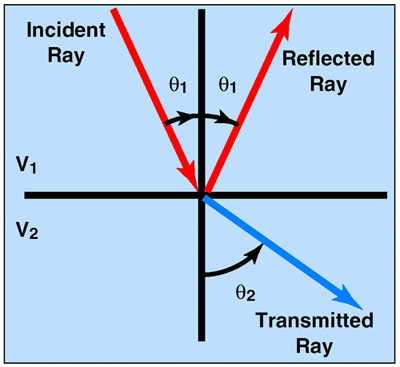
\includegraphics[width=0.4\textwidth]{snell}
%	\caption{. \label{fig:snell}} 
\end{figure}

 \begin{equation}
	\label{eq:snell}
	n_1 \cdot \sin \theta_1 = n_2 \cdot \sin \theta_2
\end{equation}

\section{\sf Construções Geométricas em Lentes Delgadas (aproximação paraxial}

\subsection{\sf Aproximações}

\subsubsection{\sf Lentes Delgadas}
Um Lente é considerada \textbf{delgada} quando a sua largura, $d$, é desprezavél façe à sua distância focal $d << f$.
\subsubsection{\sf Aproximação paraxial}
Feixes inclinados em relação ao eixo óptico de lente de um ângulo $\alpha$ , tal que
$\sin \alpha \approx \alpha$, e \\
 $\tan \alpha \approx \alpha\,$, com $\alpha < 0.1\,rad \sim 5^oº $

\begin{minipage}[c]{0.45\textwidth}
	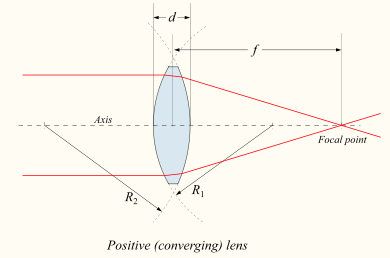
\includegraphics[width=\textwidth]{thinLens}
\end{minipage}
\begin{minipage}[c]{0.45\textwidth}
	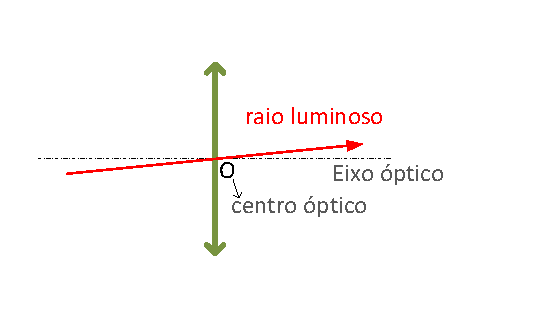
\includegraphics[width=\textwidth]{paraxial}
\end{minipage}

%\begin{figure}[!htb]  \centering 
%	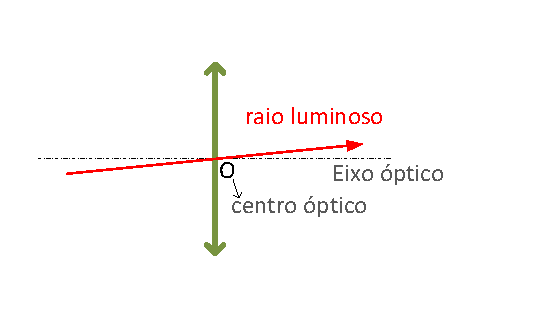
\includegraphics[width=0.7\textwidth]{paraxial}
%	\label{fig:paraxial}
%\end{figure}

\subsection{\sf Focos e Imagens}

%\begin{figure}	[!htb]  
{\centering 
	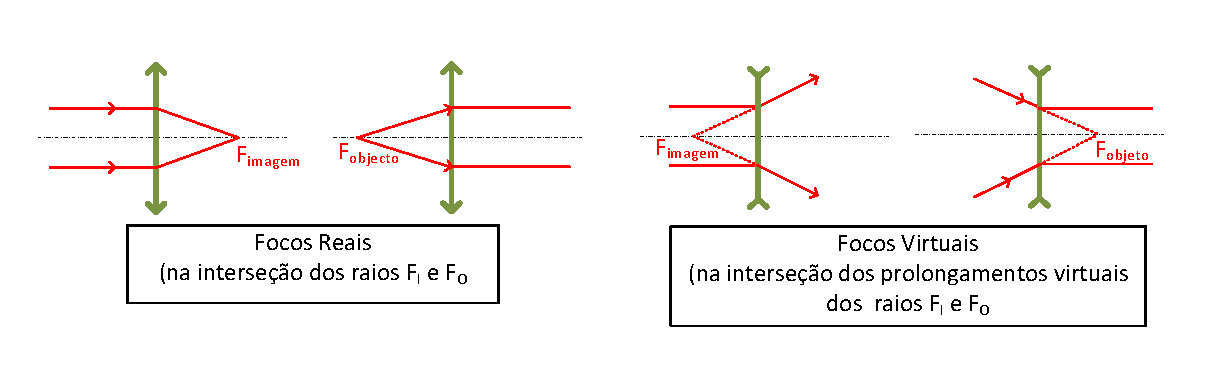
\includegraphics[width=\textwidth]{focoseImagem}
	}
%	\caption{. \label{fig:focoseImagem}} 
%\end{figure}

Nas imagens Reais o raios de luz passam de facto na posição da imagem e são as únicas que podem ser projetadas no ecrân. As imagens Virtuais, os raios parecem que vêm a imagem mas não passam nela e  são geralmente visíveis através da Lente.
\subsection{\sf Objeto e Imagem - Focos Conjungados}

\begin{figure}
	[!htb]  \centering 
	\includegraphics[width=\textwidth]{focosconjugados}
%	\caption{. \label{fig:focosconjugados}} 
\end{figure}

Pela semelhança de triângulos.
\begin{IEEEeqnarray}{rClrCl}
%\begin{array}{ccccc}
\Delta ABF_O \sim \Delta ODF_O  &\to & AB/A'B' = AF_O / F_O 0 &\to & AB/A'B' =  \frac{d_0-f}{ f} \label{eq:1} \\
\Delta ABO\sim \Delta A'B'O    &\to & AB/A'B' = AO / O A' &\to & AB/A'B' = d_O / d_I \label{eq:2} \\
\Delta COF_I \sim \Delta A'B'F_I  &\to & AB/A'B' = OF_I / F_I A' &\to & AB/A'B' =  \frac{f}{ d_I-f} \label{eq:3} 
\end{IEEEeqnarray}

de (\ref{eq:1}) e (\ref{eq:3}) obtemos a equação dos focos conjugados:
 
 \begin{equation}
	\label{eq:focosconjug}
    \fbox{
        $ \displaystyle
	\frac{1}{f} = \frac{1}{d_O} +\frac{1}{d_I} 
        $
    }
% \qquad \text{ equação dos focos conjugados}
\end{equation}



$AB$ e $A'B'$ são respetivamente as dimensões lineares transversais do objeto e da imagem  e define-se \textbf{ampliação transversal}, $A$:

$A =  \frac{A'B'}{ AB} $ que pode ser calculada por $A_{calc}=\frac{d_I}{d_O} $ atendendo a (\ref{eq:2})

No caso da última figura, $d_O > 0\;; \quad d_I > 0\,; \quad f > 0$ e a imagem é \textbf{real} e \textbf{invertida}.

\subsubsection{\sf Lente Convergente -  Imagem Real}
É fácil provar que para o funcionamento de uma máquina fotográfica  \fbox{$0 < A \le 1$ }:
(a imagem é posicionada no sensor da camera)

\begin{equation}
\infty > d_O \ge 2 f \quad \to \quad f > d_I \ge 2 f  
\end{equation}

e na montagem de um projetor de cinema ou de imagem de computador  \fbox{$1 \ge A < \infty$}:

\begin{equation}
f < d_O \le 2 f  \quad \to  \quad  2 f \le d_I < \infty 
\end{equation}

\subsubsection{\sf Lente Convergente - Imagem Virtual}
Para objetos reais a imagem é sempre virtual.
\subsubsection{\sf Funcionamento de uma Lupa}

\begin{figure}
	[!htb]  \centering 
	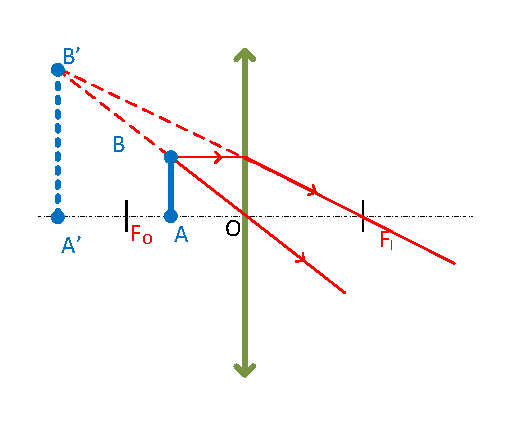
\includegraphics[width=0.8 \textwidth]{lupa}
%	\caption{. \label{fig:lupa}} 
\end{figure}

\begin{IEEEeqnarray}{rCl}
0 < d_O \le \frac{f}{2} \qquad & -f \le d_I < 0 \quad& -2 \le A < -1\\
\frac{f}{2} \le d_O < f \qquad& -\infty < d_I \le -f \quad& -\infty < A \le -2
\end{IEEEeqnarray}

\subsubsection{\sf Lente Divergente -  Imagem Virtual}

\begin{figure}
	[!htb]  \centering 
	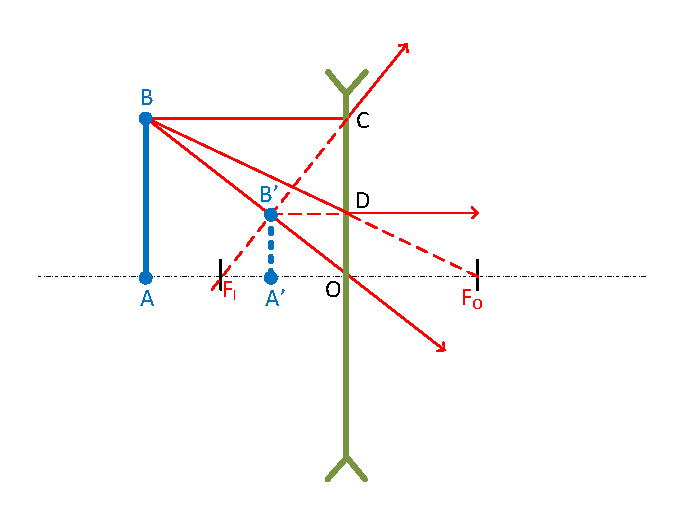
\includegraphics[width=0.8\textwidth]{diverg}
%	\caption{. \label{fig:lupa}} 
\end{figure}

$A'B'$ é uma imagem  \textbf{virtual}  e \textbf{direita} com $d_I <0$ (imagem do mesmo lado do objeto).
\begin{equation*}
f<0 \quad \to   d_O> 0 ; \quad  d_I <0  
\end{equation*}

A equação (\ref{eq:focosconjug}) pode ser obtida também pela semelhança de triângulos:

\begin{IEEEeqnarray}{rClrCl}
%\begin{array}{ccccc}
\Delta ABO \sim  \Delta A'B'O  & \to & AB/A'B' = \frac{d_0}{d_I} & \to & -\infty < A < 0 \label{eq:diver1} \\
\Delta ABF_0\sim \Delta DOF_O   &\to & \frac{d_0 + f}{f} = AB/A'B' & \to & \frac{d_0 + |f|}{|f|} = \frac{d_0 }{d_I}  \label{eq:diver2} \\
\Delta F_I C0 \sim \Delta F_I A'B'  &\to & \frac{|f|}{|f| - |d_I|} =AB/A'B'  &  \to &  \frac{|f|}{|f| - |d_I|} = \frac{d_0 }{|d_I|} 
\end{IEEEeqnarray}

As figuras construídas correspondem a objetos reais, i.e. são iluminados por luz proveniente da esquerda e 
situam-se antes da lente ($d_O > 0$).

\subsection{\sf Situação de Objetos Virtuais ($d_O<0$)}

\subsubsection{\sf Lente Convergente - Imagem Real}

\begin{minipage}[c]{0.6\textwidth}
%\begin{figure}
%	[!htb]  \centering 
	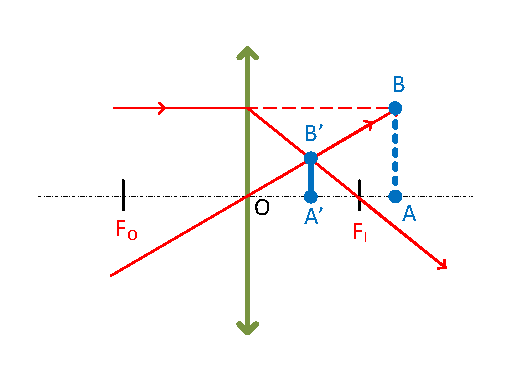
\includegraphics[width=\textwidth]{convergVirt}
%	\caption{. \label{fig:lupa}} 
%\end{figure}
\end{minipage}
\begin{minipage}[c]{0.4\textwidth}
Do objeto virtual obteve-se uma imagem \textbf{real} e \textbf{direita}.
\begin{IEEEeqnarray}{rCl}
 d_O < 0 ; \quad &&  f > 0   \nonumber\\
\frac{d_I}{-|d_O|}  & =&  \frac{f}{-|d_O| -f}     \nonumber
\end{IEEEeqnarray}
\end{minipage}

\subsubsection{\sf Lente Divergente - Imagem Virtual}

\begin{IEEEeqnarray}{rCl}
 d_O < 0 & &  f < 0   \nonumber\\
\frac{d_I}{-|d_O|}  & =&  \frac{|f|}{-|d_O| -|f|}     \nonumber
\end{IEEEeqnarray}

\begin{figure}
	[!htb]  \centering 
	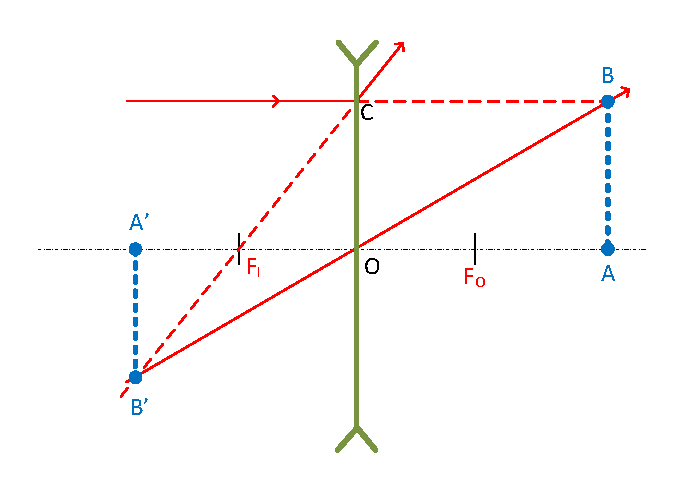
\includegraphics[width=0.7\textwidth]{divergVirt_I}
%	\caption{. \label{fig:lupa}} 
\end{figure}

Conclui-se que no caso de uma lente divergente com um objeto virtual que 
a imagem também é virtual e invertida: 
\begin{equation}
|d_O|  =  \left\{
\begin{array}{rl}
|d_O|   = |f|:  &   |d_I| \to \infty, \quad A \to \infty ,\\
|f| < |d_O|   < 2|f|:  &   |d_I|  <0 , \quad A  >1  ,\\
|d_O|   = 2|f|:  &   |d_I| = 2|f|, \quad A =1  ,\\
|d_O|  > 2|f|:   & |d_I|  <0 , \quad A  <1  .
\end{array}  \right.
%f<0 \quad \to   d_O> 0 ; \quad  d_I <0  
\end{equation}

\subsubsection{\sf Lente Divergente - Imagem Real}
\begin{IEEEeqnarray}{rCl}
\textrm{Se } d_O < 0 ; \quad  |d_O| <  |f|; \quad  |d_O| <  x|f| ; \quad (x < 1) & \to &    d_I >0; \quad A > 1 \nonumber
\end{IEEEeqnarray}


\begin{minipage}[c]{0.7\linewidth}
	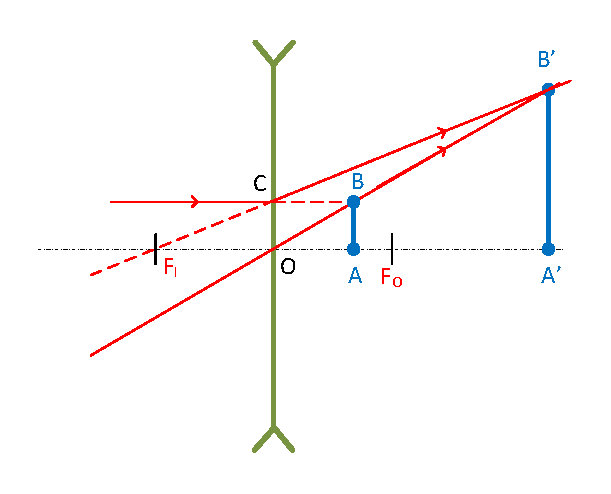
\includegraphics[width=0.7\textwidth]{divergReal}
\end{minipage}
\begin{minipage}[c]{0.3\linewidth}
A imagem é \textbf{real} e \textbf{direita}
\end{minipage}

%\begin{figure}	[!htb]  \centering 
%	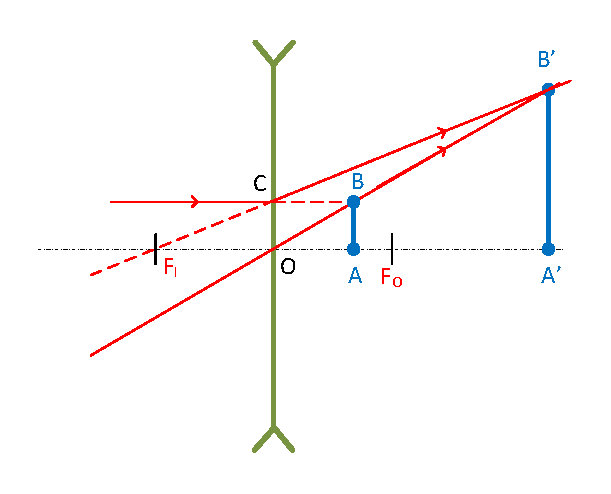
\includegraphics[width=\textwidth]{divergReal}
%	\caption{. \label{fig:lupa}} 
%\end{figure}

\subsection{\sf Associação de Lentes delgadas}

Para duas lentes delgadas de distâncias focais $f_1$ e $f_2$ afastadas de $D$ pode calcular-se a distância focal equivalente do conjunto através de 

 \begin{equation}
	\label{eq:assoclentes}
    \fbox{
        $ \displaystyle
	\frac{1}{f_{equiv}} = \frac{1}{f_1} + \frac{1}{f_2} - \frac{D}{f_1 \,f_2} 
        $
    }
\end{equation}

A dificuldade, quando se usa o método direto quer dos focos conjugados, para a determinação da distância focal equivalente, ${f_{equiv}}$ é a medida das distâncias $d_O$ e $d_I$ 
(que são diferentes das distância do objeto e de imagem às superfícies das lentes ou ao seu planos médio.

É preferível usar a equação (\ref{eq:focosconjug}) para cada uma das lentes, e considerar que a primeira imagem (real ou virtual) irá constituir-se como o “objeto”  para a segunda lente. 

Vejamos o gráfico em diferentes posições.

\subsubsection{\sf Duas lentes Convergentes afastadas de $D$}
\begin{figure}	[!htb]  \centering 
	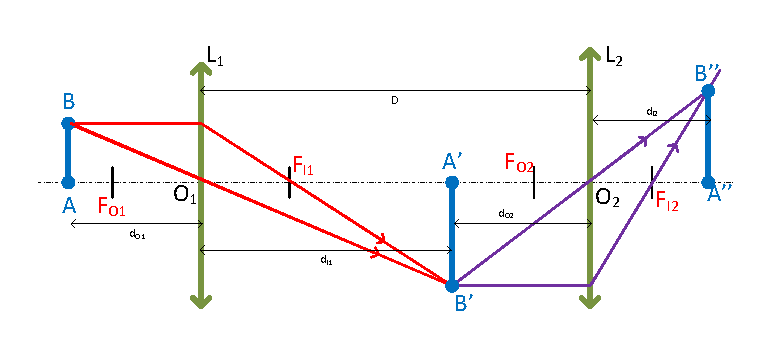
\includegraphics[width=\textwidth]{duplaConver_I}
%	\caption{. \label{fig:lupa}} 
\end{figure}

\begin{equation}
|d_O|  =  \left\{
\begin{array}{llll}
 \frac{1}{d_{O_1}} +  \frac{1}{d_{I_1}}   = \frac{1}{f_1}  & d_{O_1} = AO_1 & d_{I_1} = O_1A' & f_1 = O_1 F_{O_1} = O_1\,F_{I_1} ,\\
 \frac{1}{d_{O_2}} +  \frac{1}{d_{I_2}}   = \frac{1}{f_2}  & d_{O_2} = A'O_2 & d_{I_2} = O_2\,A'' & f_2 =  F_{O_2}\,O_2\, = O_2\,F_{I_2}, \\
O_1\,O_2 = D = d_{I_1} + d_{O_2}.
\end{array}  \right.
\label{eq:assoclentes_2}
\end{equation}

Esta é a montagem mais simples de um \textbf{telescópio}, a partir do qual se podem obter grandes ampliações.
Estas 3 expressões permitem calcular $f_2$, conhecidos os valores de $f_1$, $d_{O_1}$, $d_{I_2}$ e $D$.

No caso de uma imagem obtida por a uma lente, $L_1$, que passa a ser um “objeto” virtual para $L_2$.
\begin{figure}	[!htb]  \centering 
	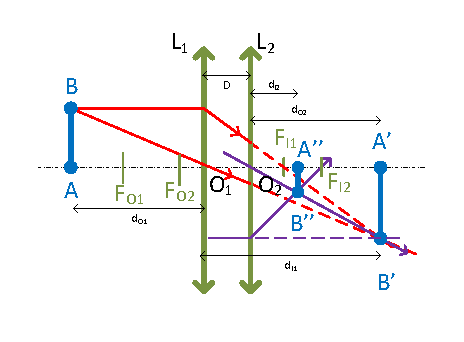
\includegraphics[width=0.8\textwidth]{duplaConver_II}
\end{figure}

\newpage
\subsubsection{\sf Lentes Convergente e Divergente afastadas de $D$}

\begin{figure}	[!htb]  \centering 
	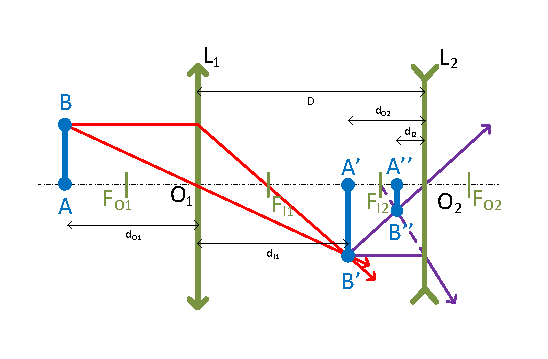
\includegraphics[width=0.8\textwidth]{ConverDiverg_I}
%	\caption{. \label{fig:lupa}} 
\end{figure}

Obtém-se uma imagem virtual produzida pela lente $L_2$ divergente a partir de imagem real obtida a partir da lente $L_1$

Na figura seguinte obtém-se uma imagem real $A''\,B''$ produzida pela lente $L_2$ divergente a partir de imagem  obtida a partir da lente $L_1$, que sua vez é um objeto virtual para a lente $L_2$

%\begin{figure}	[!htb] 
\begin{center}
	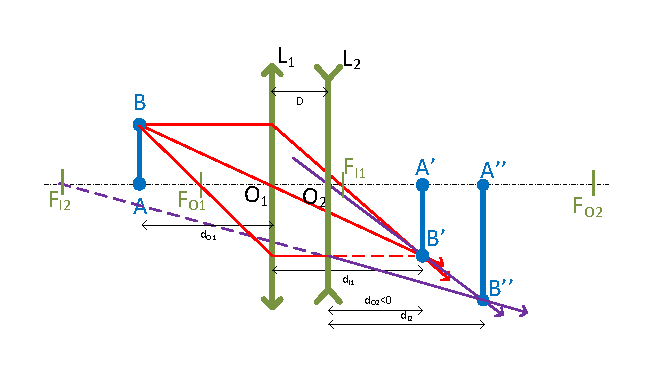
\includegraphics[width=0.8\textwidth]{ConverDiverg_II}
\end{center}

%	\caption{. \label{fig:lupa}} 
%\end{figure}


Se as lentes permutarem (Figura seguinte) obtem-se também uma imagem real  $A''\,B''$ se a distância $A\,O_1$ for semalhante nos 2 casos.
Em qualquer destas situações pode sempre calcular-se $f_2 < 0$ usando o conjunto das 3 equações (\ref{eq:assoclentes_2})

%\begin{figure}	[!htb]  
\begin{center}
	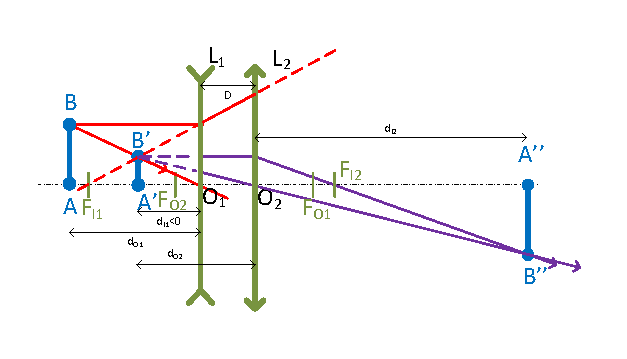
\includegraphics[width=0.8\textwidth]{ConverDiverg_III}
\end{center}
%	\caption{. \label{fig:ConverDiverg_III}} 
%\end{figure}

\subsubsection{\sf Questões a responder ANTES da sessão de Laboratório:}
\begin{enumerate}
\item Utilizando uns óculos graduados (se não usar, peça a um colega), obtenha e registe a sua graduação. Calcule a distância focal, $f=1/Dioptrias$ (para miopia são lentes divergentes, para hipermetropia são convergentes. Ignore  a correção do astigmatismo).
\item Classifique as imagens visualizadas através das lentes, i.e: Reais/Virtuais, Direitas/Invertidas, Ampliadas/Reduzidas, Posição da Imagem relativa aos objetos.
\item Para uma lente de $-2.5$ Dioptrias calcule a posicão da imagem para um objeto a 40 cm da lente. A que distância está do objeto?
\item Para uma lente convergente (óculos ou uma lupa) em que condições obtém uma imagem virtual: a) direita; b) invertida?
\end{enumerate}

\newpage
\section{\sf Protocolo Experimental}
\subsection{\sf Material utilizado}
Caixa de Óptica equipada com calha graduada, lentes convergentes e divergente, semi-cilindro de 
vidro acrílico, diafragmas, polaroides, suportes. Fonte luminosa com lâmpada de incandescência. 

\subsection{\sf Procedimento Experimental}
\subsubsection{\sf   Distância focal de uma lente convergente ( $f  ≈  75\, mm$ ) }
 
a)  Utilizando  a  fonte  luminosa  obtenha  um  feixe  de  luz  branca  de  raios  paralelos.
Determine  a  distância  focal  da  lente.  Repita  a  experiência  duas  vezes,  colocando  a  lente 
noutra posição relativamente à fonte de raios paralelos. 
b) Com a mesma lente e utilizando um feixe luminoso divergente faça uma montagem que 
lhe permita, utilizando a equação dos focos conjugados, calcular a distância focal da lente. 
Determine a ampliação linear obtida produzida pelo sistema. Compare-a com a que podia 
calcular. 
Repita a experiência duas vezes, colocando a lente noutra posição relativamente ao objeto. 
Verifique  se  a  ampliação  experimental  obtida  para  um  objeto  vertical  ou  horizontal  é  a 
mesma.  
Compare o valor da distância focal com o obtido em a) e estime a precisão envolvida em 
cada um dos métodos que utilizou. 

\subsubsection{\sf   Distância focal de uma lente divergente ( $f  ≈  -150\, mm$ ) }
Associe  no  mesmo  suporte  a  lente  divergente  com  uma  convergente  de  forma  que  o 
conjunto se comporte como um sistema convergente, por exemplo com a lente convergente 
usada em 1. Repita a montagem usada em 1b. 

Repita a experiência (pelo menos uma vez), colocando o conjunto das lentes noutra posição 
relativamente ao objeto. 
A  partir  das  distâncias  do  objeto  e  da  imagem  a  cada  uma  des  lentes  mais  próximas, 
conhecidas  a  distância  focal  da  lente  convergente  e  a  distância  entre  lentes,  calcule  a 
distância focal da lente divergente. 

\subsubsection{\sf  Índice de refracção dum vidro acrílico }

Faça  incidir  luz  branca  na  superfície  plana  do  semi-cilindro  de  vidro  acrílico.  Observe  a 
reflexão e a transmissão de modo a produzir a reflexão, relativamente ao feixe incidente, à 
direita  e  depois  à  esquerda.  Faça  medições  pelo  menos  para  cinco  valores  diferentes  do 
ângulo de incidência. Determine graficamente o índice de refracção do vidro acrílico.  
Repita  as  medidas  e  a  análise  dos  resultados  fazendo  agora  a  incidência  na  superfície 
cilíndrica. Conclua sobre o índice de refracção do vidro acrílico a partir dos dois conjuntos 
de medidas. 
Estime o valor do índice de refracção a partir do ângulo limite de reflexão total. 
Compare a precisão dos diferentes valores obtidos para o índice de refracção. 

\subsubsection{\sf Polarização da luz. Ângulo de Brewster}
Observe o efeito de interposição de dois polaroides paralelos ou cruzados no percurso de 
um feixe luminoso. 
Usando a mesma montagem do ponto 3, polarize o feixe incidente paralelamente ao plano
de incidência e observe experimentalmente para valores do ângulo de incidência próximos 
do  ângulo  de  Brewster  (que  pode  calcular  a  partir  dos  resultados  que  obteve)  o  intervalo 
angular em que há praticamente extinção do feixe refletido. Observe a intensidade do feixe 
transmitido. 

\subsubsection{\sf Montagens Ópticas}
Com duas lentes convergente tente obter um telescópio (objetos distantes) e um miscroscópio simples. Desenhe a montagem, as distancias utilizadas e a Ampliação obtida.
É possível ter a Imagem final na posição do Objeto?
\end{document} 